\chapter{Final Walking Tests}
    The final walking tests are comprised of three different terrains: a simple flat plane as a baseline, then a staircase to demonstrate simple foot and body height adjustment, and finally a uneven organic like surface.

    Please note that all data is plotted with the world axis aligned to the robot's starting orientation in the world. This is done for graphing clarity.
    
    % When presenting testing data, a snapshot of the 3D simulation environment will be shown, with the body and foot paths traced. Additionally key data points
    % are also graphed, however only the height of a single foot will be graphed, this is to maintain clarity.

    \section{Flat Terrain}
    The flat plane test aims to quantify nominal body height oscillations and to provide a baseline to compare subsequent test to. Figure \ref{fig:plane_test} and \ref{fig:plane_test_top} shows screenshots of the simulation test being performed in \ac{mujoco}. A video of the simulation can be seen \href{https://youtu.be/pw4GzVp-8aQ}{\color{blue}\underline{here}}.
    \begin{figure}[h]
        \centering
        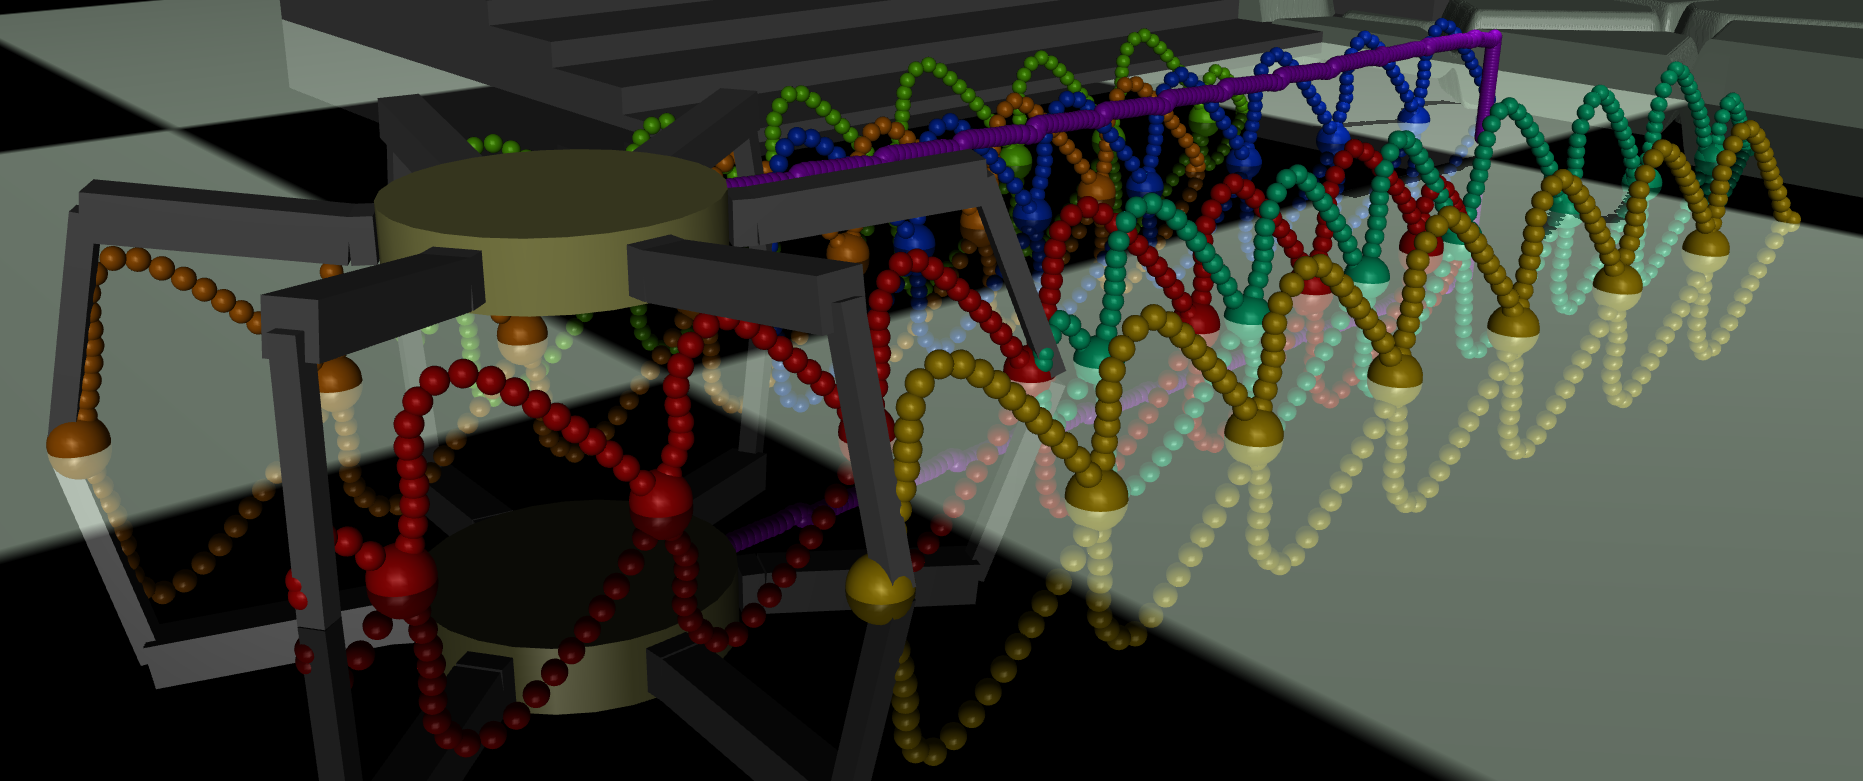
\includegraphics[width=\textwidth]{Flat.png}
        \caption{Flat terrain \ac{mujoco} view.}
        \label{fig:plane_test}
    \end{figure}

    \noindent
    The test was performed with a nominal stride length of 15cm, while the flow function parameters \(Ch\) and \(q\) were set to 2.0 and 14.0 respectively. This equates to a desired step height roughly equal to true stride length, which is dependant on the terrain. The target body height was set to \(13.5cm\) above the virtual floor height (see section \ref{sec:height_adjust}). The robot was commanded to walk forwards at a constant speed.
    \begin{figure}[h]
        \centering
        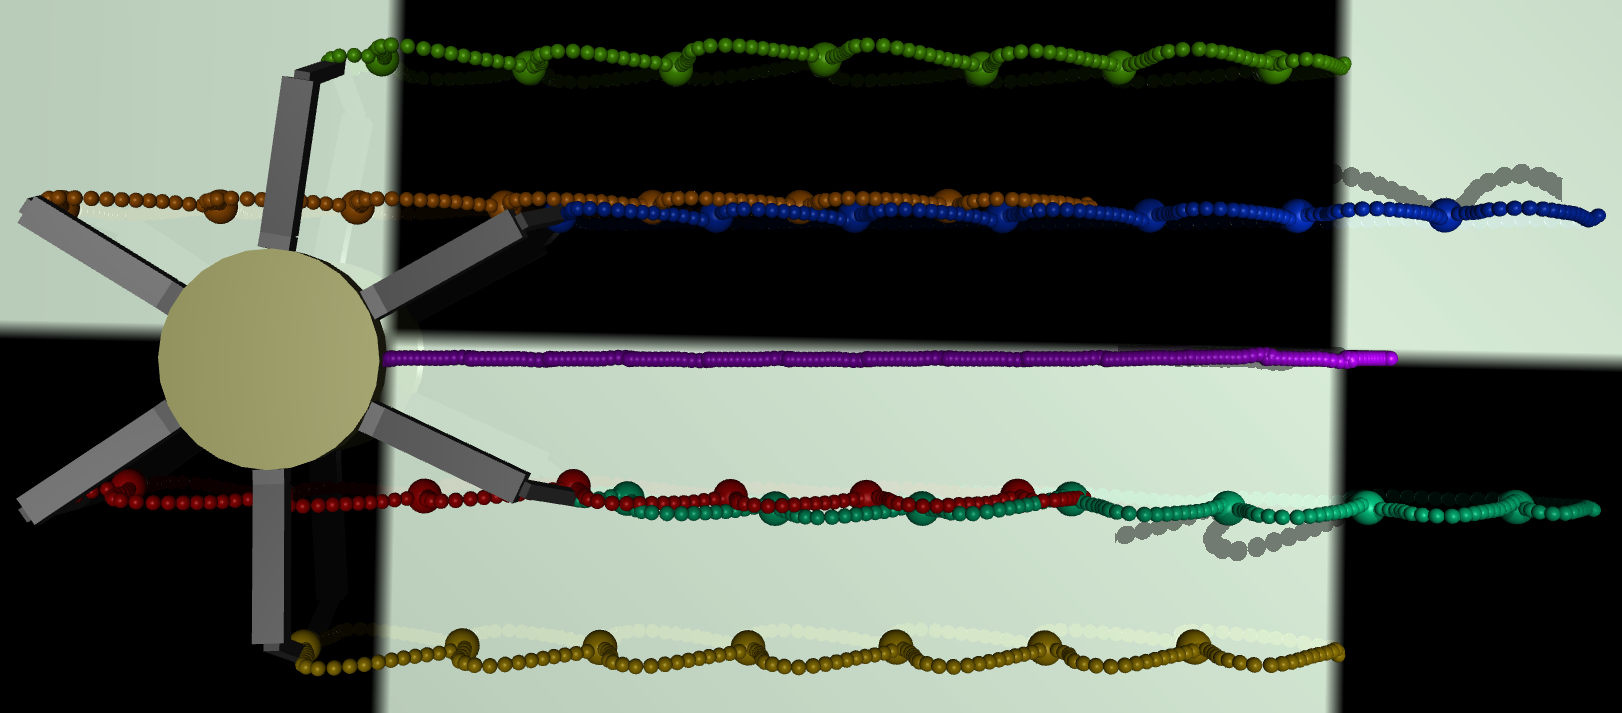
\includegraphics[width=\textwidth]{FlatTop.png}
        \caption{Flat terrain \ac{mujoco} top view.}
        \label{fig:plane_test_top}
    \end{figure}
    
    \noindent
    The simulation results for the body feet trajectories are show in Figure \ref{fig:flat_feet},
    \begin{figure}[h]
        \centering
        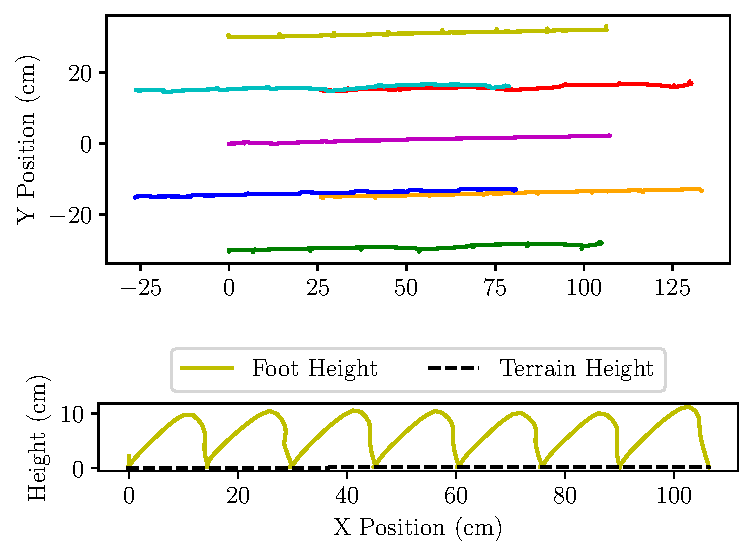
\includegraphics{flat_test_feet.pdf}
        \caption{Flat terrain. Feet top view (Top). One foot side view (Bottom).}
        \label{fig:flat_feet}
    \end{figure}

    \noindent
    where the color codes match that of the above screenshots. It can be seen that the stride length is equal to the set stride of \(15cm\). The robot also maintains a linear trajectory throughout the test. Note that the step height is about \(10cm\) which is a little lower than expected. The reason for this is that the swinging feet are being "pushed" through the flow function faster by the supporting legs faster than expected. Thus, resulting in a lower arc.

    Figure \ref{fig:flat_body} shows the body height and rotation. Here it can be seen that there is a constant error of about 1cm in the body height of the robot. The reason for this is that there is no body height feedback control, as such, errors in the servos accumulate to result in the body height error. This can be easily solved by adding a constant offset or by adding feedback control for the body height.
    \begin{figure}[h]
        \centering
        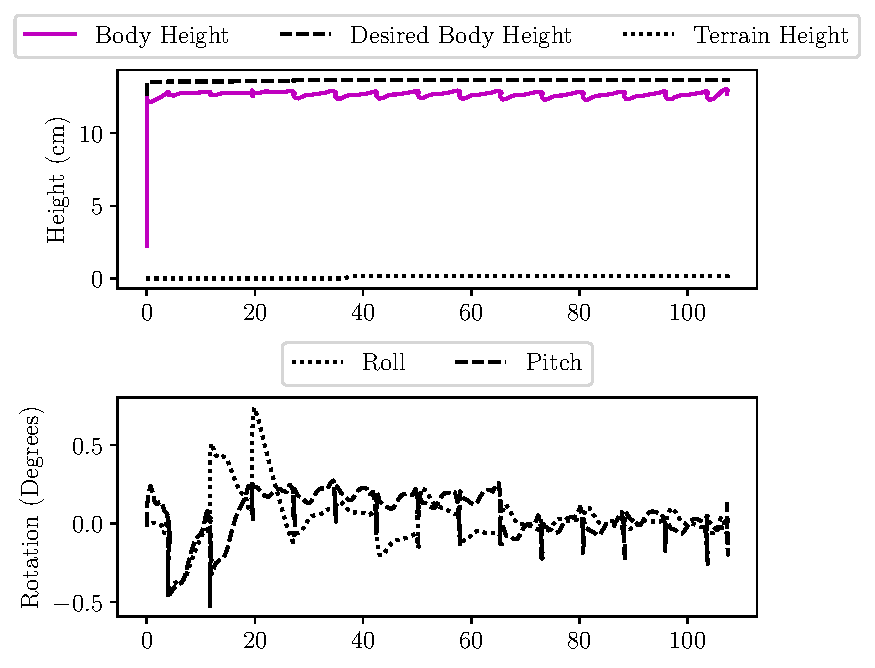
\includegraphics{flat_test_body.pdf}
        \caption{Flat terrain. Body height (Top). Body tilt (Bottom).}
        \label{fig:flat_body}
    \end{figure}
    It is also clear that as the robot walks there are some oscillations in the body height. This is to be expected as the servos are not modeled as having infinite torque, thus, the robot will sag when three legs are lifted off the ground, and rebound once those legs are placed on the floor again. Similarly to the body height error, adding feedback control on the body height would reduce these oscillations. The amplitude of the oscillations are lower than the \(10\%\) of the desired body height, which is acceptable. Next, it can be seen that the tilt of the body also exhibit small oscillations, in both roll and pitch. However, the amplitudes of these oscillations remain below 0.5 degrees.

    
    \section{Staircase}
    A staircase test was performed where the hexapod was commanded to move onto a set of steps. This tested the system's ability to choose foot placements that are not close to edges, to maintain a level body, and to automatically adjust its body height relative to the local terrain height. Figure \ref{fig:stairs} show screenshots of the test simulation in \ac{mujoco}. A video of the simulation can be found \href{https://youtu.be/6v_fmXEp1Vs}{\color{blue}\underline{here}}.
    \begin{figure}[h]
        \centering
        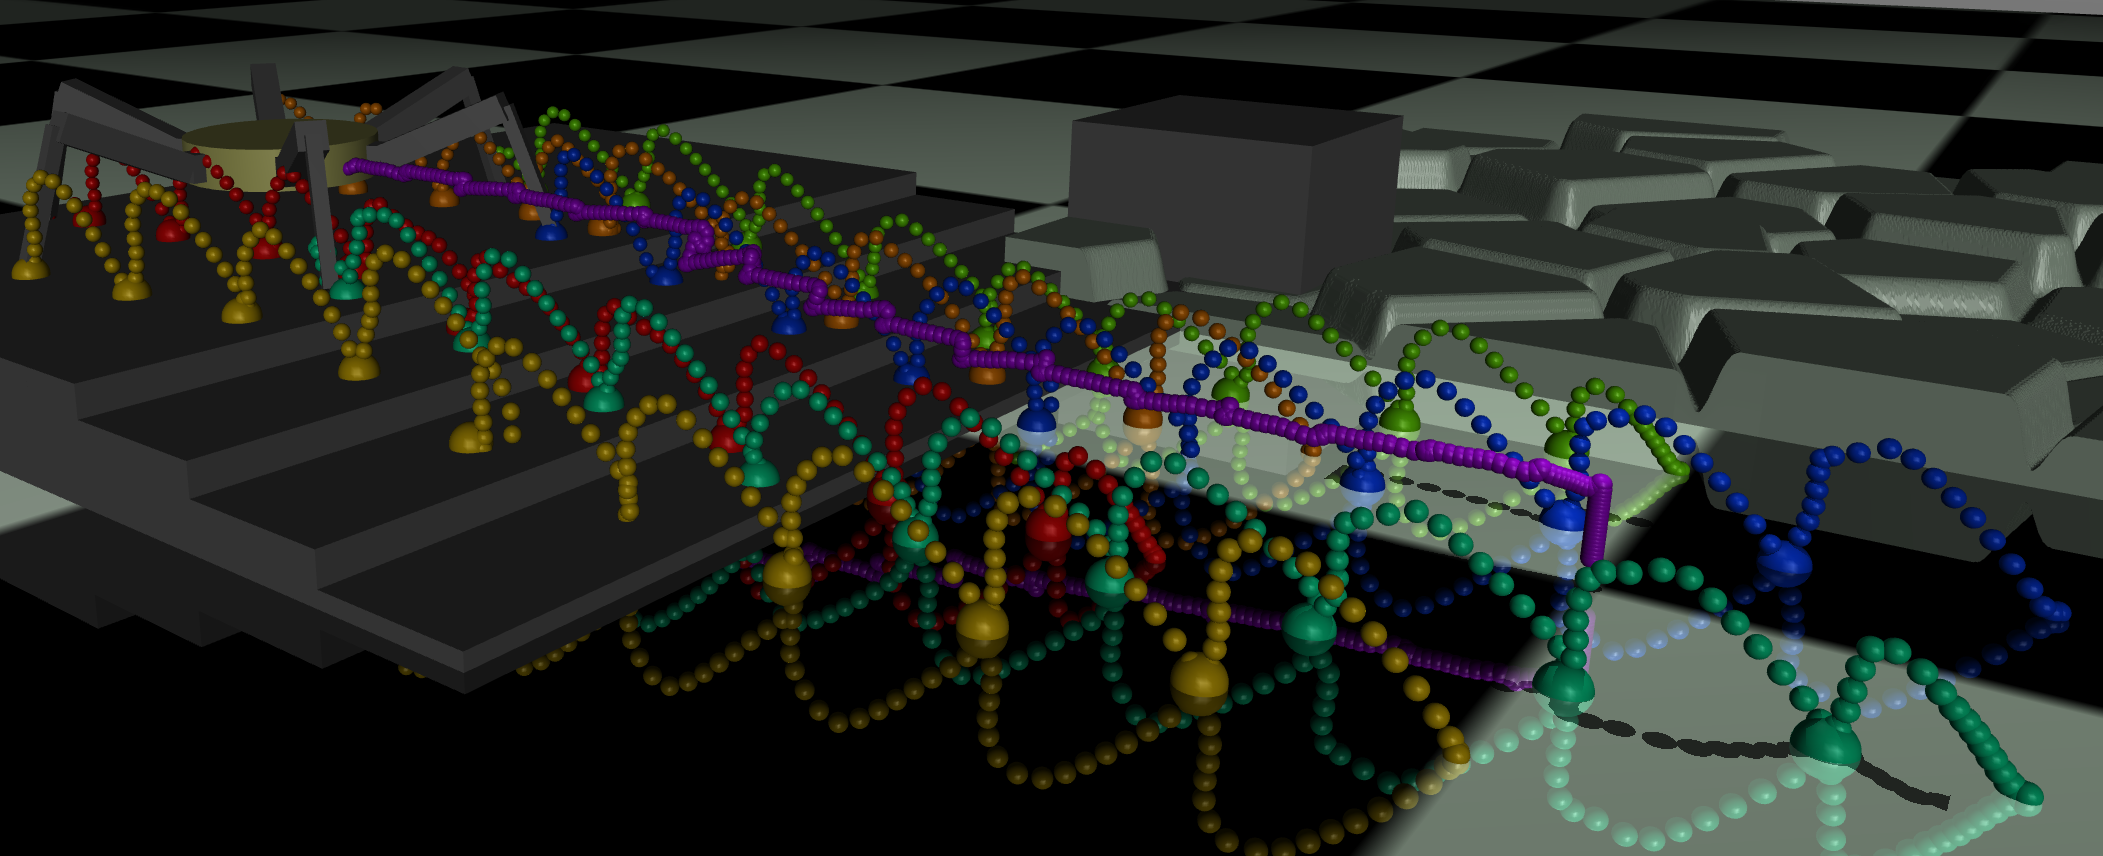
\includegraphics[width=\textwidth]{Stairs.png}
        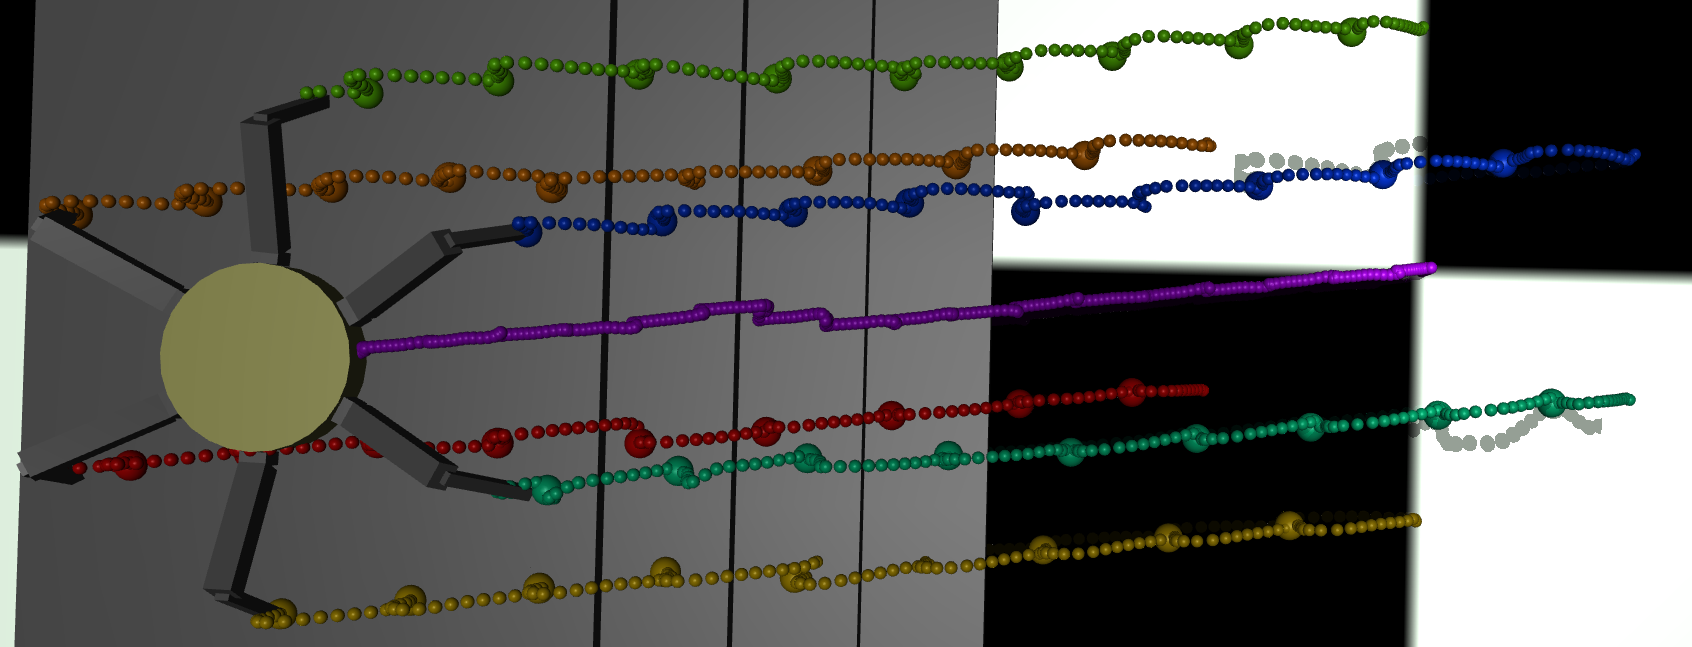
\includegraphics[width=\textwidth]{StairsTop.png}
        \caption{Stairs \ac{mujoco} view.}
        \label{fig:stairs}
    \end{figure}

    \noindent
    The test was performed with a nominal \(15cm\) stride length, the flow parameters \(Ch\) and \(q\) were set to \(2.0\) and \(14.0\) respectively. This results in a step height roughly equal to the true stride length. The target body height is set to \(9cm\) target height above the virtual floor height (see section \ref{sec:height_adjust}). The robot was commanded to walk forwards at a constant velocity.

    % \begin{figure}[h]
    %     \centering
    %     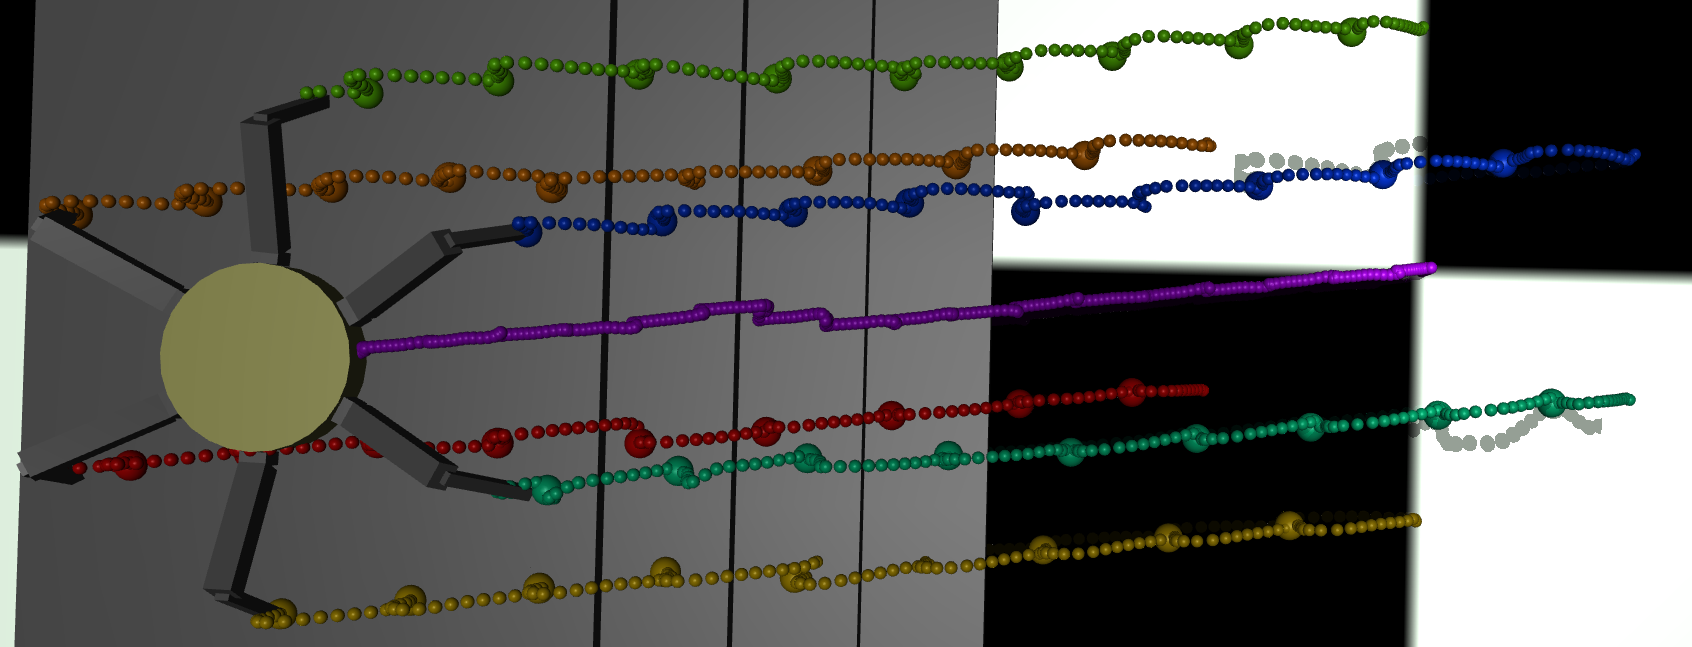
\includegraphics[width=.9\textwidth]{StairsTop.png}
    %     \caption{Stairs \ac{mujoco} view top}
    %     \label{fig:stairs_top}
    % \end{figure}
    The body and feet trajectories are show in figure \ref{fig:stairs_feet}. The robot maintains a mostly linear trajectory up the staris, with a small deviation around \(80cm\) down the X axis. The stride lenght is mostly equal to the nominal \(15cm\), however, the step starting at \(70cm\) has a visibly longer stride length, this is to avoid stepping on the edge of the step. Also note that some steps start with a small loop, this occurs when the robot bumps itself backwards with the front feet. This happens when the front feet push into the ground during a longer stride, due to the slight error in the body height. Similarly to the flat terrain test, the constant body height error is still present. 
    \begin{figure}[h]
        \centering
        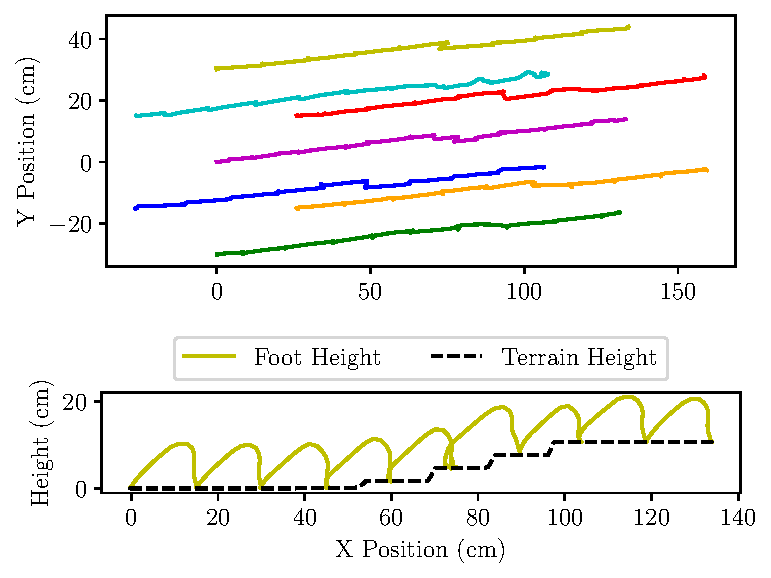
\includegraphics{stairs2_test_feet.pdf}
        \caption{Stairs. Feet top view (Top). One foot side view (Bottom).}
        \label{fig:stairs_feet}
    \end{figure}

    \noindent
    Figure \ref{fig:stairs_body} shows the body height and rotation. From this it can be seen that the robot does increase its height to maintain a constant height above the terrain. It is clear that the body height is not increased in the four discrete steps as the stairs do, rather the body height is increased more smoothly using many smaller steps. This is thanks to the system described in section \ref{sec:height_adjust}.
    The oscillations in the body tilt angles are more prominent in the staircase test than in the flat terrain test, but still mostly stay below 1 degrees, with some intermittent jumps approaching 2 degrees.
    \begin{figure}[h]
        \centering
        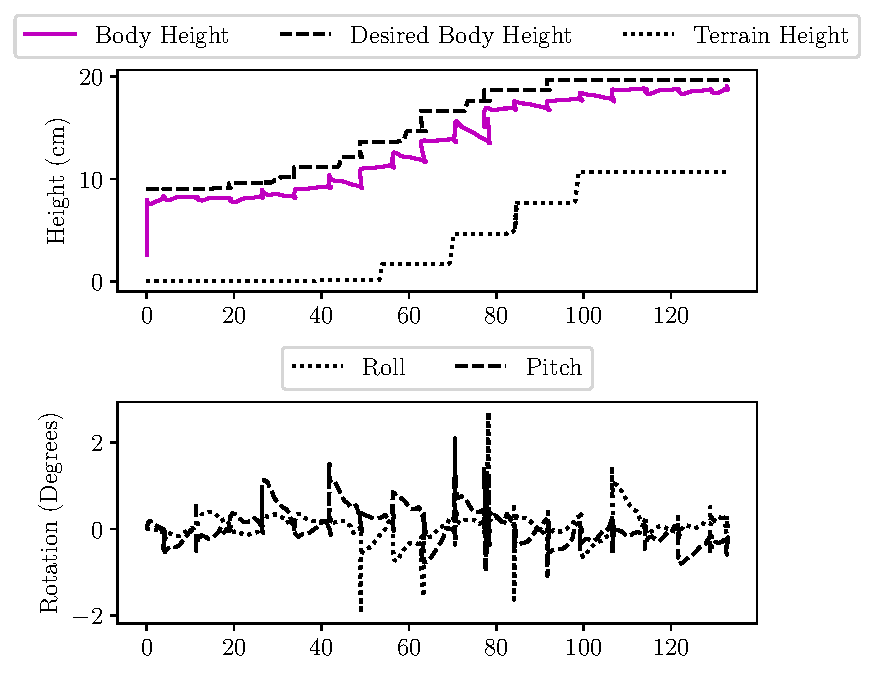
\includegraphics{stairs2_test_body.pdf}
        \caption{Stairs. Feet top view (Top). One foot side view (Bottom).}
        \label{fig:stairs_body}
    \end{figure}

    \section{Cobblestone terrain}
    An organic terrain test was performed where the hexapod was commanded to move over uneven terrain consisting of "cobblestones" with grooves between them and with varying slopes and heights. Figure \ref{fig:org_test} and \ref{fig:org_test_top} show screenshots
    \begin{center}
        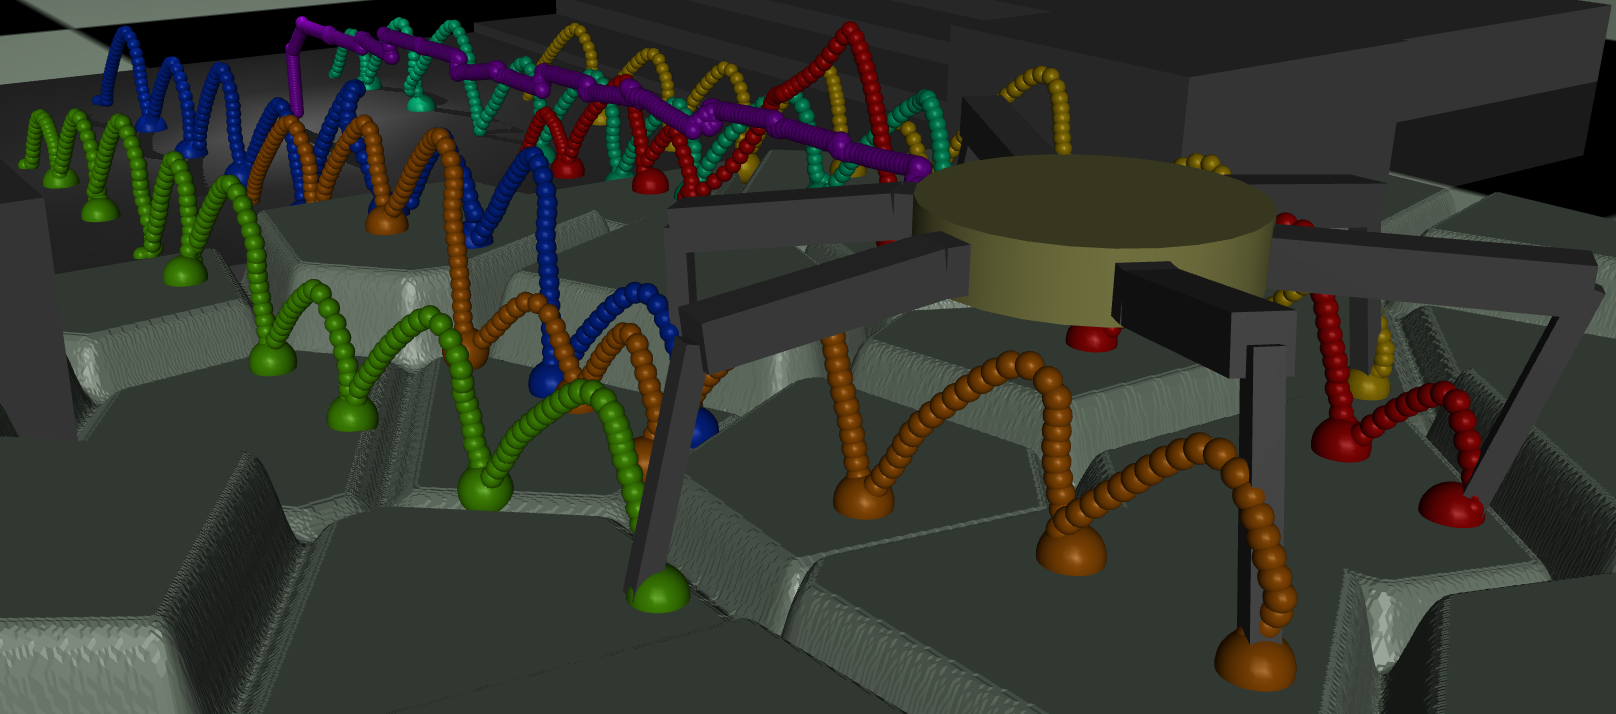
\includegraphics[width=.83\textwidth]{Cobble.png}
        \captionof{figure}{Cobblestone test \ac{mujoco} view.}
        \label{fig:org_test}
    \end{center}
    of the cobblestone test in \ac{mujoco}. A video of the simulated test can be seen \href{https://youtu.be/-lQjvykGlmY}{\color{blue}\underline{here}}. The cobblestones presented islands of suitable foot placement locations, while the grooves represented areas that are not suitable for foot placement. This tested the system's ability to choose suitable foot placements, to maintain a level body and a desired body height, and to traverse uneven terrain.
    % \captionsetup[figure]{oneside,margin={0.9cm,0cm}}
    \begin{figure}[h]
        \centering
        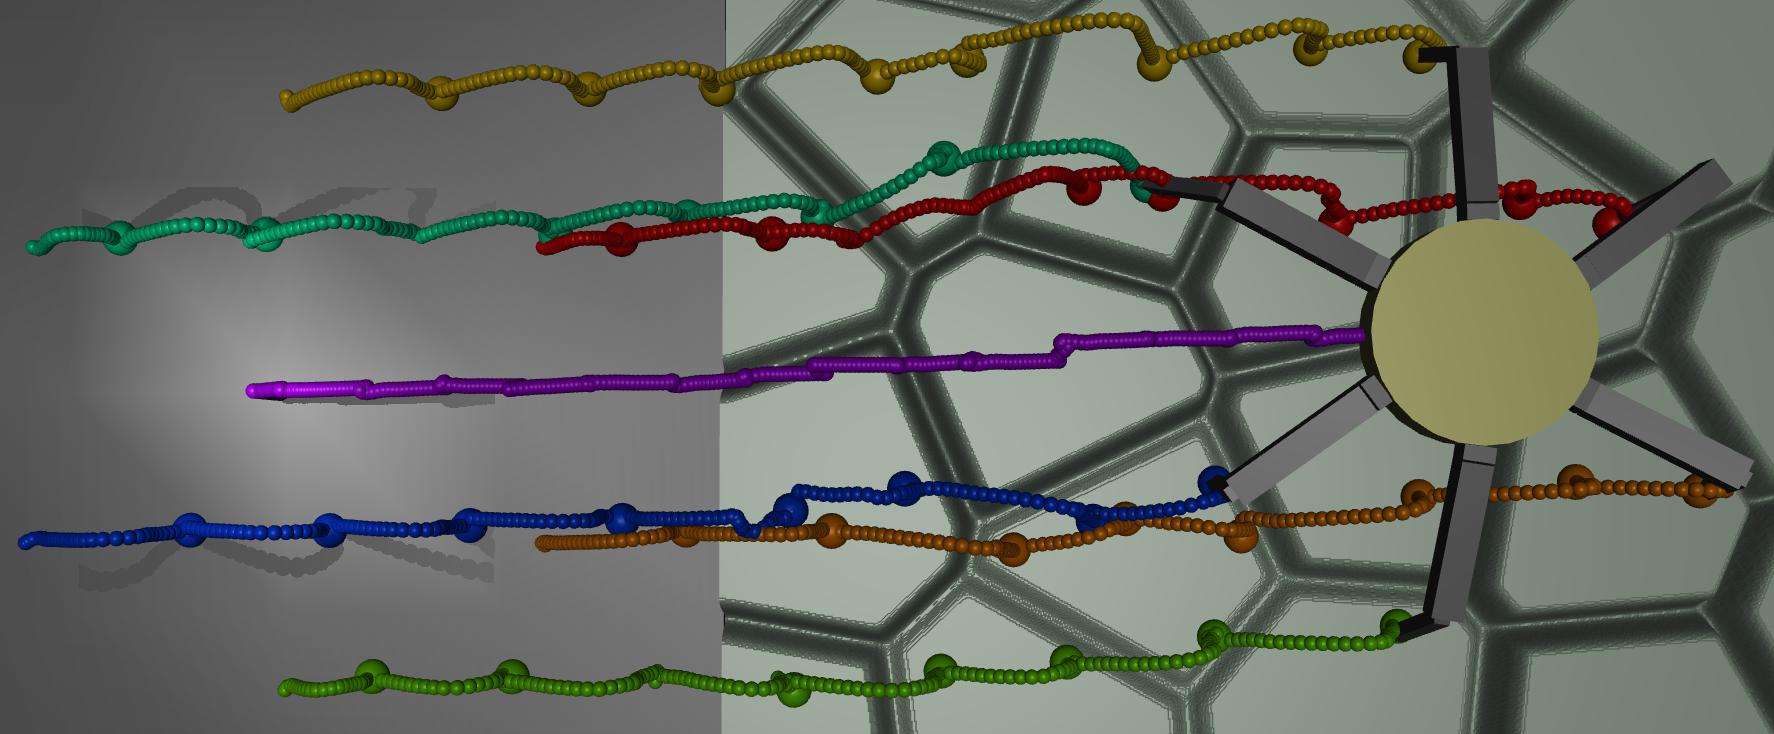
\includegraphics[width=.83\textwidth]{CobbleTop.png}
        \caption{Cobblestone test \ac{mujoco} top view.}
        \label{fig:org_test_top}
    \end{figure}

    \noindent
    Similar to past tests, the robot was commanded to walk over the terrain in a straight line at a constant velocity. The nominal stride length was set to \(15cm\) and the flow parameters \(Ch\) and \(q\) were set to \(2.0\) and \(14.0\) respectively. Figure \ref{fig:cobble_feet} shows the body and leg trajectories. The robot still maintains a straight

    \begin{centering}
        \centering
        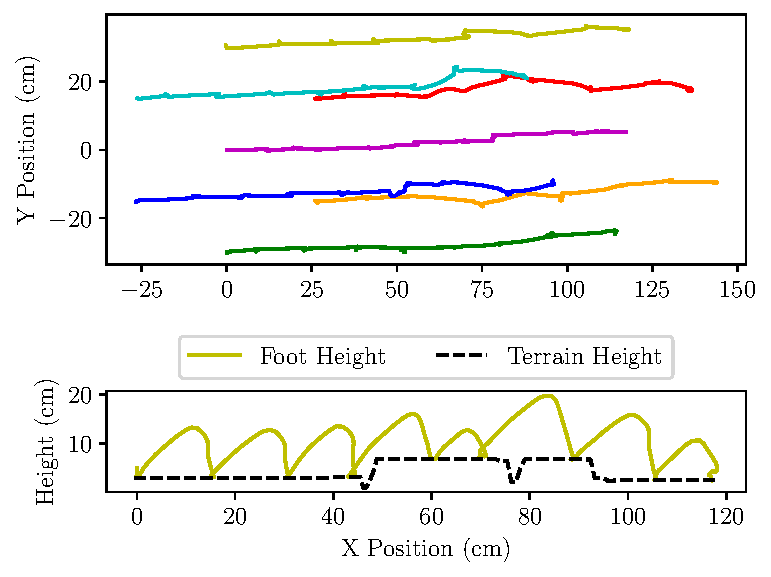
\includegraphics{cobble_test_feet.pdf}
        \captionof{figure}{Cobblestones. Feet top view (Top). One foot side view (Bottom).}
        \label{fig:cobble_feet}
    \end{centering}
    \noindent
    trajectory over the terrain. This test clearly demonstrates how the robot adjusts its feet targets in the horizontal plane to place them on the cobbles. Similarly, stride length is also greatly adjusted, as can be seen from figure \ref{fig:cobble_feet}.

    Figure \ref{fig:cobble_body} shows the body heigh and rotation during the cobblestone terrain test.
    \begin{figure}[h]
        \centering
        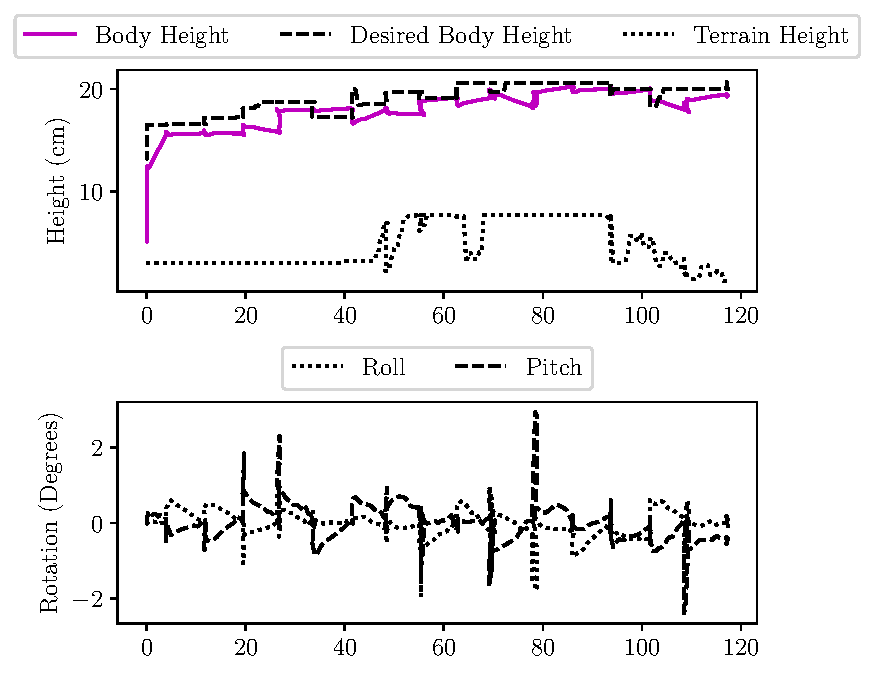
\includegraphics{cobble_test_body.pdf}
        \caption{Cobblestones. Body height (Top). Body tilt (Bottom).}
        \label{fig:cobble_body}
    \end{figure}
    From this it can be seen that the body height error seen in the flat plane test is still present, and more severe. However, the body height still stays within a reasonable margin from the desired height.

    For the most part, the oscillations in the body rotation is similar to that of the stairs test. However, they are more frequent, and more sever spikes are present. This is due, in part, to the more erratic mismatch between the body height and the requested body height. The horizontal adjustments made to the foot placement positions cause the swinging feet to end their steps at different times. This is the primary cause of the tilt spikes, as when one foot is placed on the floor before the other two, the robot is tilted slightly. This, however, would not occur if there was no, or little, error in the body height control.

    % Finally, when looking at the foot position plot in figure \ref{fig:org_test_data}, please note that the plot is a projection into the X-Z plane, and thus any adjustment made in the Y-axis is not shown, the foot shown has been chosen to include minimum Y-axis variation. Thus, please also see the 3D view in figure \ref{fig:org_test}. From these two figures it is clear that the foot end positions are, in addition to height, adjusted in the horizontal plane, the step arcs are appropriately adjusted and remain relatively smooth, similar to the flat plane test.


% \bigskip
% \bigskip
% \hrule
% \smallbreak
% \hrule
